\documentclass{article}


\usepackage{subcaption}
\usepackage{circuitikz}
\usepackage[T1]{fontenc} 
\usepackage[utf8]{inputenc}
\usepackage{amsmath}
\usepackage{amssymb}
\usepackage{fancyhdr}
\usepackage{graphicx}
\usepackage{hyperref}
\usepackage{tikz}
  \usetikzlibrary{arrows}
  \usetikzlibrary{shapes}
  \usetikzlibrary{arrows.meta,topaths}
  \usetikzlibrary{bending}
  \usetikzlibrary{calc}
\usepackage{anyfontsize}
\usepackage{sectsty}
\usepackage{../assets/scripts/tex/color-env}
\usepackage{anyfontsize}
\usepackage{xcolor}
\definecolor{DarkGreenBlue}{HTML}{264653}
\definecolor{LightGreenBlue}{HTML}{2A9D8F}
\definecolor{LightOrange}{HTML}{E9C46A}
\definecolor{DarkOrange}{HTML}{F4A261}
\definecolor{RedOrange}{HTML}{E76F51}
\definecolor{BrightRed}{HTML}{D62828}
\definecolor{DeepBlue}{HTML}{003049}



\usepackage[ngerman]{babel}
\title{Elektrotechnik 1 - Praktikum 3}


\usepackage[
  includehead,
  headheight = 17mm,
  footskip = \dimexpr\headsep+\ht\strutbox\relax,
  tmargin = 0mm,
  bmargin = \dimexpr17mm+2\ht\strutbox\relax,
]{geometry}





\pagestyle{fancy}
\fancyhead[L]{\leftmark}
\fancyhead[R]{}
\fancyfoot[L]{}
\fancyfoot[C]{\thepage}
\fancyfoot[R]{
\includegraphics[scale=0.2]{../assets/images/haw.jpg}}
\renewcommand\headrulewidth{0.5pt}

\begin{document}

\thispagestyle{empty}
\begin{tikzpicture}[remember picture,overlay]

  \fill[DeepBlue] (current page.south west) rectangle (current page.north east);

  \begin{scope}

    \foreach \i in {2.5,...,22}
      {
        \node[rounded corners, DeepBlue!90,draw ,regular polygon, regular polygon sides=6, minimum size=\i cm, ultra thick] at ($(current page.west)+(2.5,-5)$) {} ;
      }

  \end{scope}

  \node[rounded corners,fill=DeepBlue!95,text =DeepBlue!5,regular polygon,regular polygon sides=6, minimum size=2.5 cm,inner sep=0,ultra thick] at ($(current page.west)+(2.5,-5)$) {\LARGE \bfseries 2020};

  \foreach \i in {0.5,...,22}
    {
      \node[rounded corners,DeepBlue!90,draw,regular polygon,regular polygon sides=6, minimum size=\i cm,ultra thick] at ($(current page.north west)+(2.5,0)$) {} ;
    }

  \foreach \i in {0.5,...,22}
    {
      \node[rounded corners,DeepBlue!98,draw,regular polygon,regular polygon sides=6, minimum size=\i cm,ultra thick] at ($(current page.north east)+(0,-9.5)$) {} ;
    }

  \foreach \i in {12}
    {
      \node[fill = DeepBlue,rounded corners,draw=DeepBlue,regular polygon,regular polygon sides=6, minimum size=\i cm,ultra thick] at ($(current page.south east)+(-0.2,-0.45)$) {} ;
    }


  \foreach \i in {21,...,6}
    {
      \node[DeepBlue!95,rounded corners,draw,regular polygon,regular polygon sides=6, minimum size=\i cm,ultra thick] at ($(current page.south east)+(-0.2,-0.45)$) {} ;
    }

  \node[left,DeepBlue!5,minimum width=0.625*\paperwidth,minimum height=3cm, rounded corners] at ($(current page.north east)+(0,-9.5)$){{\fontsize{25}{30} \selectfont \bfseries ET2 - Praktikum 6}};

  \node[left,DeepBlue!10,minimum width=0.625*\paperwidth,minimum height=2cm, rounded corners] at ($(current page.north east)+(0,-11)$){{\huge \textit{Simulation Transienter Vorgänge}}};

  \node[left,DeepBlue!5,minimum width=0.625*\paperwidth,minimum height=2cm, rounded corners] at ($(current page.north east)+(0,-13)$){{\Large \textsc{Florian Tietjen\hspace{0.5cm}Eric Antosch}}};

\end{tikzpicture}

\newpage
\thispagestyle{empty}

\tableofcontents


\newpage

\section{Vorbereitung}
\subsection{Schaltvorgang einer RC-Reihenschaltung}
Es seien $R_{1}$ und $C_{1}$ in Reihe geschaltet und über einen Schalter mit einer Gleichspannungsquelle von $U_{1} = 60V$ verbunden. Zum Zeitpunkt $t_{0} = 0ms$ wird der Schalter geschlossen, es sei dabei $R_{1} = 2k\Omega$ und $C_{1} = 10\mu F$. Der Strom über das RC-Glied ist durch $I = \frac{U_{1}}{R_{C}} = \frac{60V}{2k\Omega} = 30mA$ gegeben.
Wir berechnen dazu zunächst $\tau = R_{1} \cdot C_{1} = 2k\Omega \cdot 10\mu F = 0,02 s$. Damit können wir nun mit der folgenden Formel die gefragten Werte berechnen:
\begin{equation}
  \label{eq:1}
  u_{C}(t) = U_{0} + \Delta U \cdot e^{-\frac{t}{\tau}} = U_{0} + (U_{C,t_{0}} - U_{0})\cdot e^{-\frac{t}{\tau}}
\end{equation}
\begin{equation}
  \label{eq:2}
  i_{C}(t) = \frac{u_{C}(t)}{R_{C}}
\end{equation}
\subsubsection{Anfangs ungeladener Kondensator $u_{C}(0ms) = 0V$}
Damit können wir nun die Werte für $u_{C}(t_{1})$ und $i_{C}(t_{1})$ berechnen, wobei $t_{1} = 12ms$ gilt.

\begin{equation*}
  u_{C}(t_{1}) = U_{0}+\Delta U \cdot e^{-\frac{t}{\tau}} = 60V + -60V \cdot e^{-\frac{12ms}{20ms}} = 27,071V.
\end{equation*}
\begin{equation*}
  i_{C}(t_{1}) = \frac{U_{0}}{R_{C}} \cdot e^{-\frac{t}{\tau}} = \frac{60V}{2k\Omega} \cdot e^{-\frac{12ms}{20ms}} = 0,01646A.
\end{equation*}

\begin{figure}[h]
\centering
    \begin{subfigure}[b]{0.4\textwidth}
    \centering
    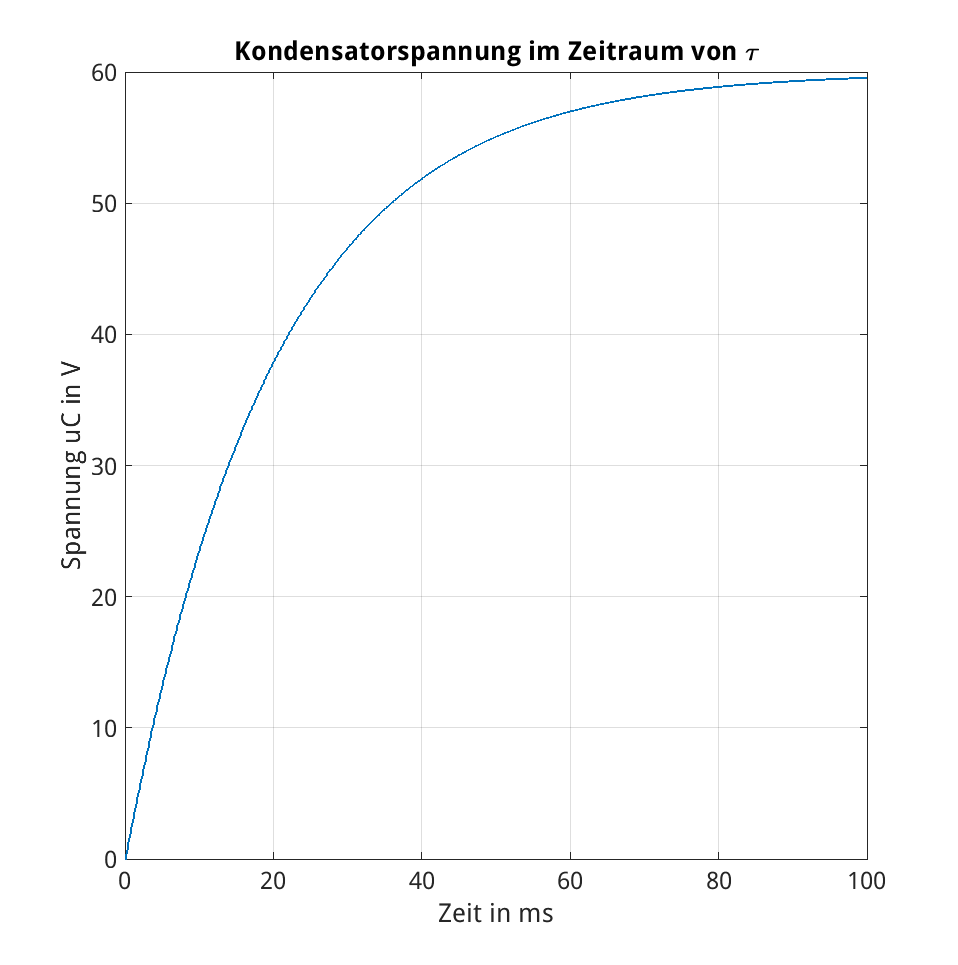
\includegraphics[width=\textwidth]{../assets/images/ET2P5/Kondensatorspannung11.png}
    \caption{Aufladespannungskurve des Kondensators}
  \end{subfigure}
  \hfill
  \begin{subfigure}[b]{0.4\textwidth}
    \centering
    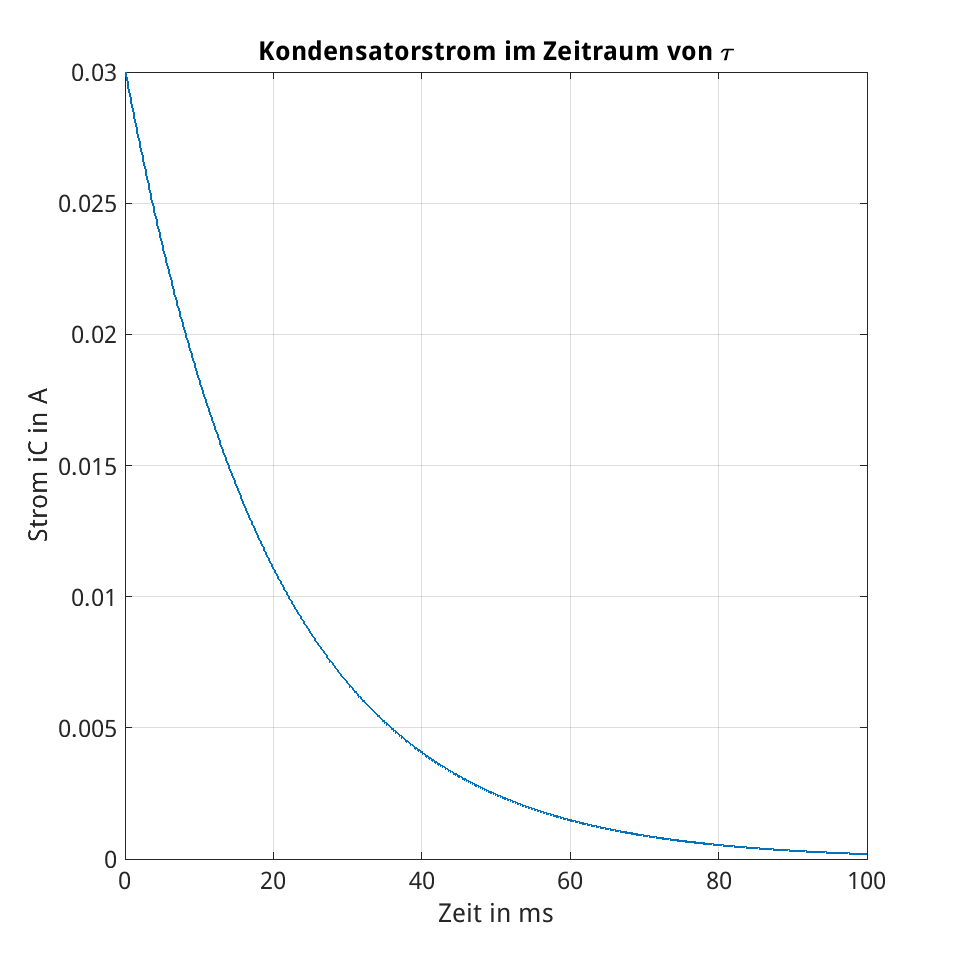
\includegraphics[width=\textwidth]{../assets/images/ET2P5/Kondensatorstrom11.png}
    \caption{Aufladestromkurve des Kondensators}
  \end{subfigure}

  \caption{Kondensatorspannung für a) im Zeitraum $\tau$}
  \label{fig:con1}
\end{figure}

\subsubsection{Anfangs geladener Kondensator $u_{C}(0ms) = 10V$}

Mit (\ref{eq:1}) berechnen wir nun die Spannung über den Kondensator durch:
\begin{equation*}
  u_{C}(t_{1}) = U_{0}+\Delta U \cdot e^{-\frac{t}{\tau}} = 60V + -50V \cdot e^{-\frac{12ms}{20ms}} = 32,559V
  i_{C}(t_{1}) = \frac{\Delta U}{R_{C}} \cdot e^{-\frac{t}{\tau}} = 25mA \cdot e^{-\frac{12ms}{20ms}} = 13,72mA
\end{equation*}

Mit den oben gezeigten Formeln ergeben sich dementsprechend folgende Zeitverläufe:

\begin{figure}[h]
\centering
    \begin{subfigure}[b]{0.4\textwidth}
    \centering
    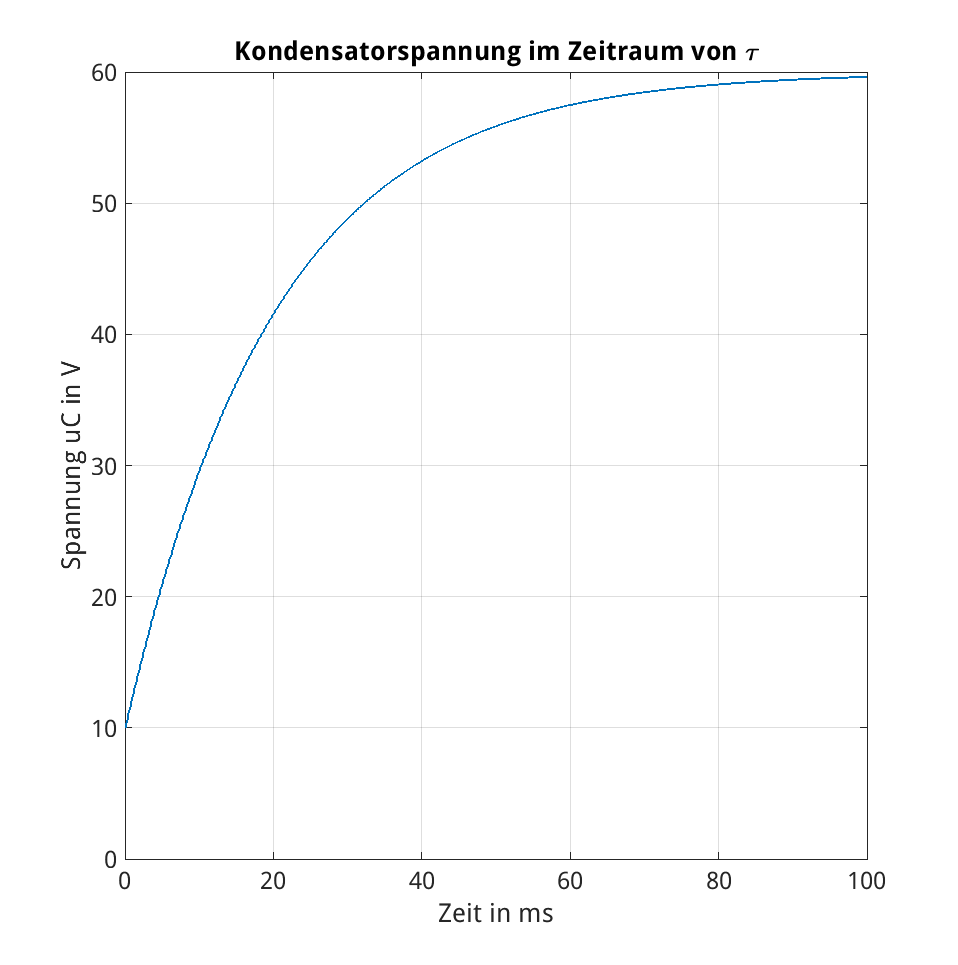
\includegraphics[width=\textwidth]{../assets/images/ET2P5/Kondensatorspannung12.png}
    \caption{Aufladespannungskurve des Kondensators}
  \end{subfigure}
  \hfill
  \begin{subfigure}[b]{0.4\textwidth}
    \centering
    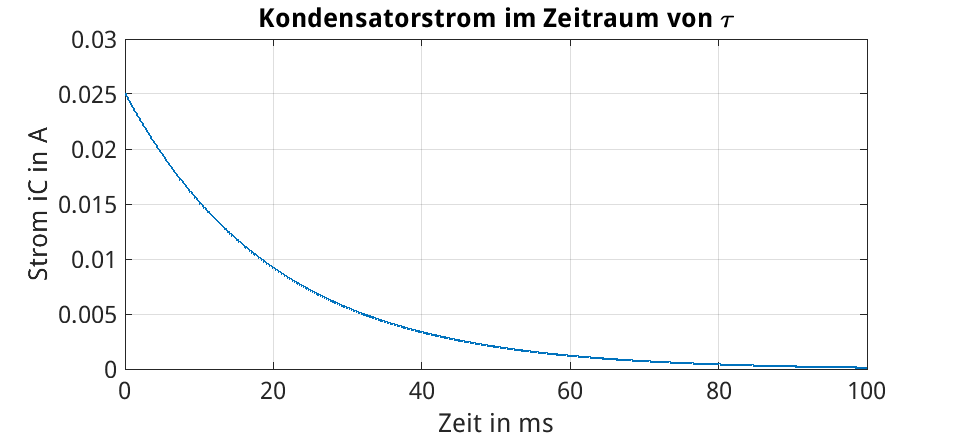
\includegraphics[width=\textwidth]{../assets/images/ET2P5/Kondensatorstrom12.png}
    \caption{Aufladestromkurve des Kondensators}
  \end{subfigure}

  \caption{Kondensatorspannung für b) im Zeitraum $\tau$}
  \label{fig:con1}
\end{figure}


\subsection{Schaltvorgang bei einem Netzwerk mit einem Kondensator (ein Schaltzeitpunkt)}

\begin{figure}[h]
  \begin{center}
    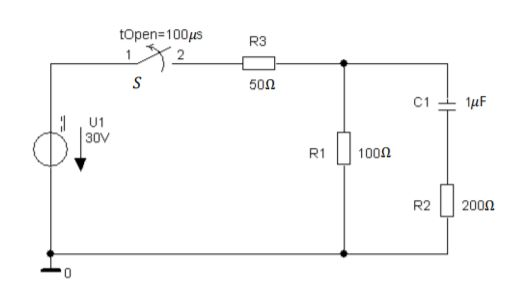
\includegraphics[scale=1]{../assets/images/ET2P5/vorbereitung 2.jpg}
    \caption{Versuchsaufbau des Netzwerkes}
  \end{center}
\end{figure}

Zunächst soll die Anfangsspannung am Kondensator $u_C$ (0) bestimmt werden:

\begin{align*}
  u_C(0) &= U_{R1} = \frac{R1}{R1+R3} \cdot U1 \\
  u_C(0) &= \frac{100\Omega}{100\Omega + 50\Omega} \cdot 30V = 20V
\end{align*}

Nun wird die Spannung am Kondensator für den eingeschwungenen Zustand $u_C$ (t) für $t \rightarrow \infty$ berechnet:
\begin{align*}
  u_C(t)&= U_0 \cdot e^{-\frac{t}{RC}} = 0V
\end{align*}

Bestimmung der Zeitkonstante $\tau$ für geschlossenen Schalter:
\begin{align*}
  \tau &= RC = ((R3 // R1) + R2) \cdot C = 33\mu s
\end{align*}

Bei geöffnetem Schalter:
\begin{align*}
  \tau &= RC = (R1 + R2) \cdot C = 300\mu s
\end{align*}

Daraus ergeben sich die allgemeinen Formeln für den zeitlichen Verlauf der Spannung und des Stroms für alle t >= $100\mu s$

\begin{align*}
  u_C(t)&= 20V \cdot e^{-\frac{t-100\mu s}{300\mu s}}\\
  i_C(t)&= -66,7mA \cdot e^{-\frac{t-100\mu s}{300\mu s}}
\end{align*}

\newpage

\subsection{Schaltvorgang bei einem Netzwerk mit einem Kondensator (zwei Schaltzeitpunkt)}

\begin{figure}[h]
  \begin{center}
    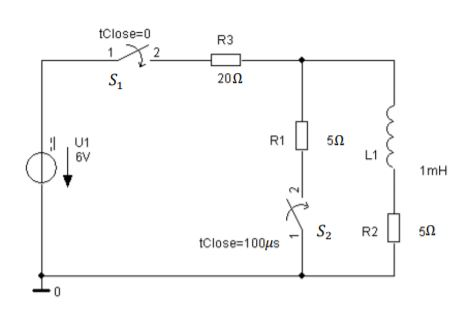
\includegraphics[scale=1]{../assets/images/ET2P5/vorbereitung 3.jpg}
    \caption{Versuchsaufbau des Netzwerkes}
  \end{center}
\end{figure}

Die folgende Schaltung ist das Ersatzschaltbild für $t0 < t < t1$:
\begin{figure}[h]
  \begin{center}
    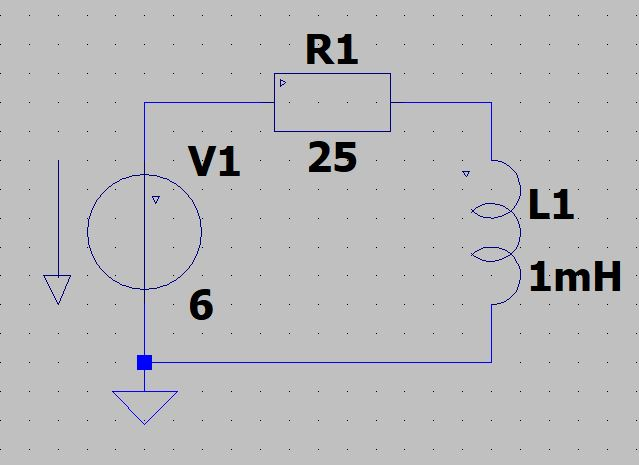
\includegraphics[scale=0.3]{../assets/images/ET2P5/t0 t t1.JPG}
    \caption{ESB für $t0 < t < t1$ }
  \end{center}
\end{figure}

Die folgende Schaltung ist das Ersatzschaltbild für $t1 < t$:
\begin{figure}[h]
  \begin{center}
    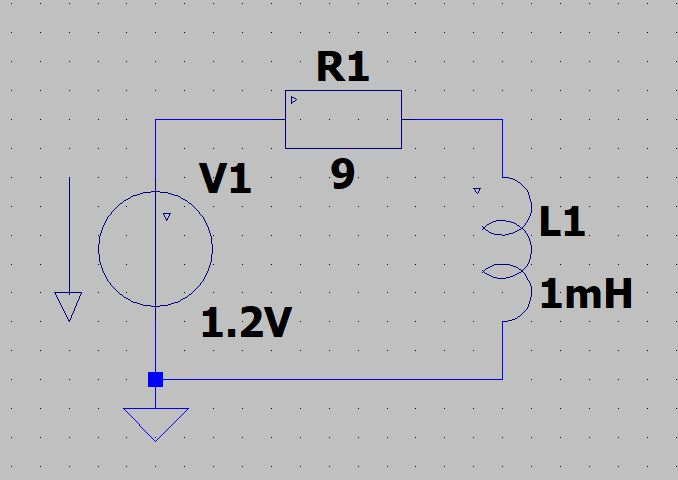
\includegraphics[scale=0.3]{../assets/images/ET2P5/t1 kleiner t.JPG}
    \caption{ESB für $t1 < t$ }
  \end{center}
\end{figure}
\newpage

Berechnung des Stroms $i_{L1}$ für $t_0$:
\begin{align*}
  i_{L1} = 0A
\end{align*}
Da die Spule anfangs wie ein unendlicher hoher Widerstand wirkt, ist der Strom bei $t_0$ 0A.\\


Für $i_{L1}$, wenn $t \rightarrow \infty$ und S2 stets geöffnet ist, gilt:
\begin{align*}
  i_{L1}&= i_{R_g} = \frac{U1}{R_g} = \frac{6V}{25\Omega}\\
  i_{L1}&= 240mA
\end{align*}
Dabei wurde die Spule wie kurzgeschlossen betrachtet. \\

Die Zeitkonstanten für $t_0 < t < t_1$ ergibt sich aus:
\begin{align*}
  \tau_{t0} &= \frac{L1}{R} = \frac{1mH}{25\Omega}=40\mu s
\end{align*}

Gleichung für den Spulenstrom $i_L$ lautet:
\begin{align*}
  i_{L1}(t) = 240mA (1 - e^{-\frac{t}{40\mu s}})\\
  i_{L1}(t=t_1=100\mu) = 220mA
\end{align*}

Für die Zeitkonstante sowie für den Strom wenn beide Schalter geschlossen sind für $t \rightarrow \infty$ gilt:
\begin{align*}
  \tau = \frac{L}{R} = \frac{L}{(R1//R3)+R2} = \frac{1mH}{9\Omega} = 111,1\mu s\\
  t\rightarrow\infty : i_L(t) = 133,33mA
\end{align*}

Da sich die Spule ab t = $100\mu s$ wieder entlädt gilt:
\begin{align*}
  i_{L1}(t1=100\mu) - i_{L1}(t=t\rightarrow \infty) &= 220mA - 133,33mA = 86,67mA\\
  i_{L1}(t) &= 133,33mA + 86,67mA\cdot e^{-\frac{t-100\mu s}{111,1\mu s}})
\end{align*}


Lösen des Stroms nach $200\mu$s:
\begin{align*}
  i_{L1}(t=200\mu s) &= 133,33mA + 86,67mA\cdot e^{-\frac{t-100\mu s}{111,1\mu s}})\\
  i_{L1}(200\mu s) &= 168,69mA
\end{align*}

\newpage
\section{Schaltvorgang einer RC-Reihenschaltung}

\begin{task}
  T
  In diesem Versuch wollen wir den Schaltvorgang einer RC-Reihenschaltung mithilfe von LTSpice simulieren und anschließend untersuchen. Dazu verwenden wir genau zum einen einen ungeladenen Kondensator und zum anderen einen vorgeladenen Kondensator mit $u_{C}(0ms) = 10V$.
\end{task}

Wir stellen unsere Simulation der Aufgabe entsprechend mit folgenden Werten für den Schalter
\begin{itemize}
  \item ttrans = $1\mu s$
  \item tClose = 0ms
  \item Rclosed = $0,01\Omega$
  \item Ropen = $1M\Omega$
\end{itemize}
und für die Transient Analysis
\begin{itemize}
  \item Print step = 0
  \item Stop time = 100ms
  \item Step Ceiling(Timestep) = 0.01
  \item Skip initial transient solution = disabled(diese Einstellung existiert in LTSpice so nicht mehr)
\end{itemize}
ein.

\subsection{Anfangs ungeladener Kondensator $u_C(0ms)=0V$}
\label{sec:anfangs-ungel-kond}


Nach dem Einschalten der Schaltung bei LTSpice ergeben sich folgende Verläufe für Strom und Spannung:

\begin{figure}[h]
  \begin{center}
  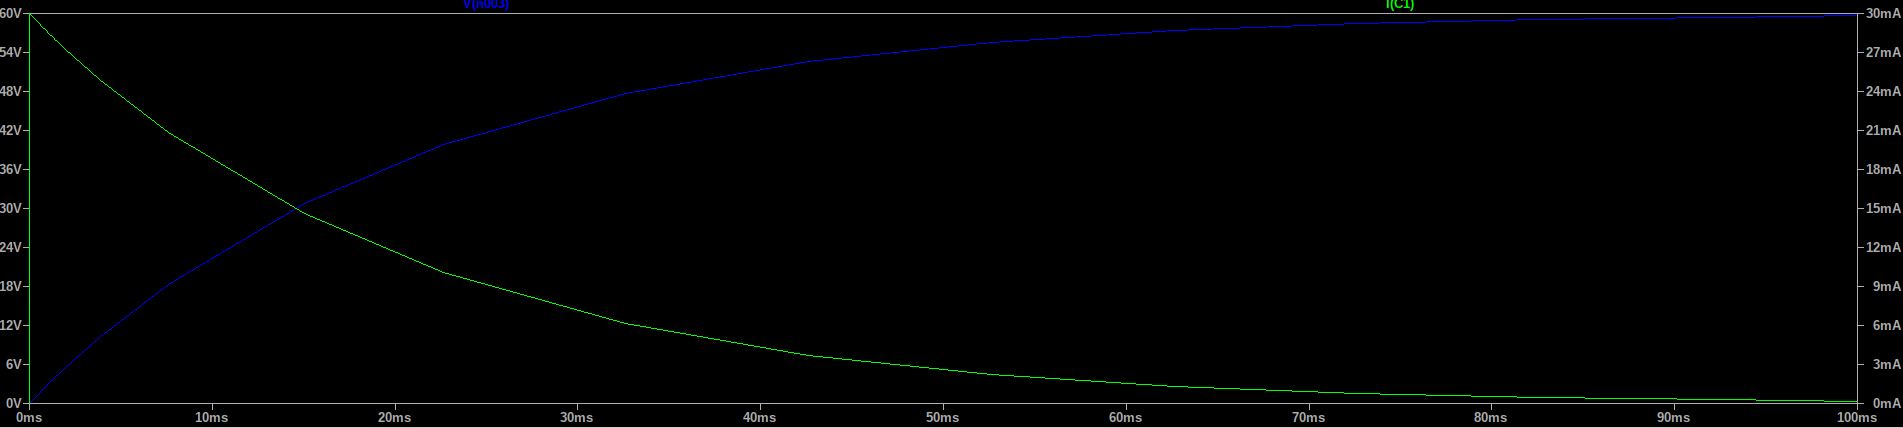
\includegraphics[scale=0.32]{../assets/images/ET2P5/StromSpannung11.png}
  \caption{Strom- und Spannungsverlauf der Simulation mit LTSpice von a)}
\end{center}
\end{figure}
\newpage



Mithilfe der Cursorfunktion ermitteln wir den Wert $\tau_{1} = 20,84ms$:

\begin{figure}[h]
  \centering
  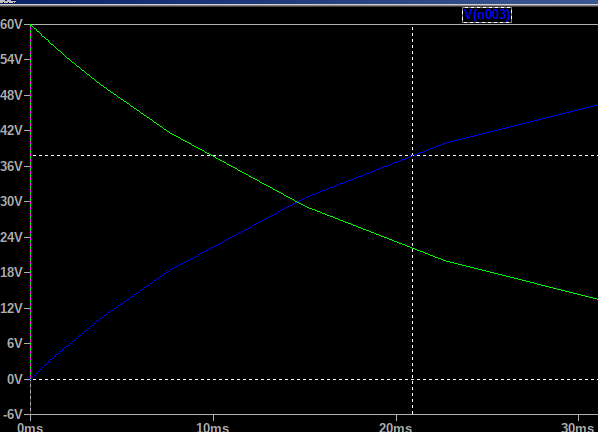
\includegraphics[scale=0.5]{../assets/images/ET2P5/Zeitkonstante11.png}
  \caption{Cursorfunktion zur Ermittlung der Zeitkonstante $\tau_1$}
  \label{fig:cont11}
\end{figure}

Wir erkennen damit sehr genau, dass der Zeitverlauf der Kurve ziemlich genau mit der Kurve in der Vorbereitung übereinstimmt, auch die Abweichung der Zeitkonstante $\tau_{1}$ ist sehr gering. Sie entsteht hier durch die annäherung der Schaltereigenschaften in der Simulation, die wir in unserer Rechnung nicht berücksichtigt haben.


\subsection{Anfangs geladener Kondensator $u_C(0ms)=10V$}
\label{sec:anfangs-gelad-kond}

Nach dem Einschalten der Schaltung bei LTSpice ergeben sich folgende Verläufe, die sehr stark an den Verlauf oben erinnern, wobei hier ein Offset von 10V zu bemerken ist:

\begin{figure}[h]
  \centering
  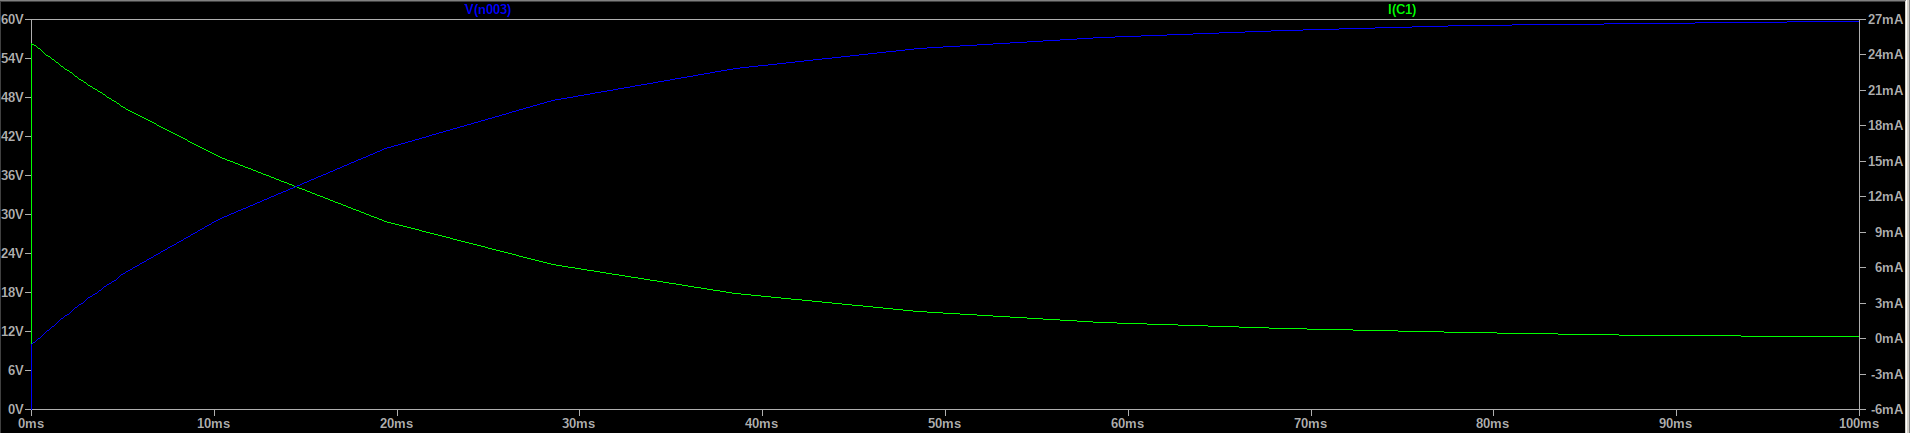
\includegraphics[scale=0.32]{../assets/images/ET2P5/StromSpannung12.png}
  \caption{Strom- und Spannungsverlauf der Simulation mit LTSpice von b)}
  \label{fig:con12}
\end{figure}

Mithilfe der Cursorfunktion ermitteln wir wieder erneut die Zeitkonstante $\tau_{2} = 19,48ms$:

\begin{figure}[h]
  \centering
  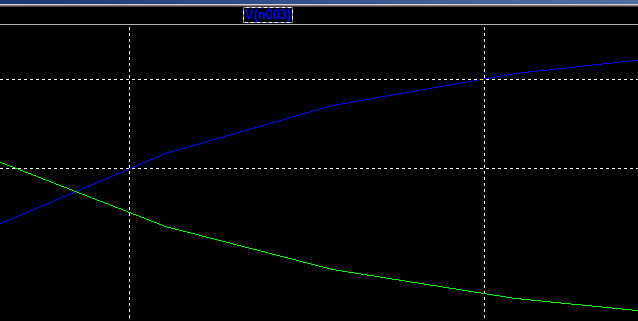
\includegraphics[scale=0.5]{../assets/images/ET2P5/Zeitkonstante12.png}
  \caption{Cursorfunktion zur Ermittlung der Zeitkonstante $\tau_2$}
  \label{fig:cont12}
\end{figure}

Aus der Ermittlung der Zeitkonstanten für den vorgeladenen Kondensator erkennen wir zwar erneut, dass die Zeitkonstante sehr nahe an der theoretisch genutzen Zeitkonstante liegt, jedoch in die negative Richtung abweicht. Das lässt aus der Vorladung des Kondensator herleiten, der dem Prozess des vollständigen Aufladens die Eigenschaft verleiht, weniger Zeit zu brauchen, da schon ein Teil der zu erreichenden Ladung vorhanden ist.

\newpage

\section{Schaltvorgang bei einem Netzwerk mit einem Kondensator (ein Schaltzeitpunkt)}
\begin{task}
  T
  In diesem Versuch wollen wir das Verhalten eines Kondensators in einem Netzwerk untersuchen, der durch einen Schalter gesteuert ist. Dazu verwenden wir LTSpice, um den Sachverhalt so genau wie möglich zu simulieren.
\end{task}
\subsection{Simulation der Schaltung}
\begin{figure}[h]
  \begin{center}
    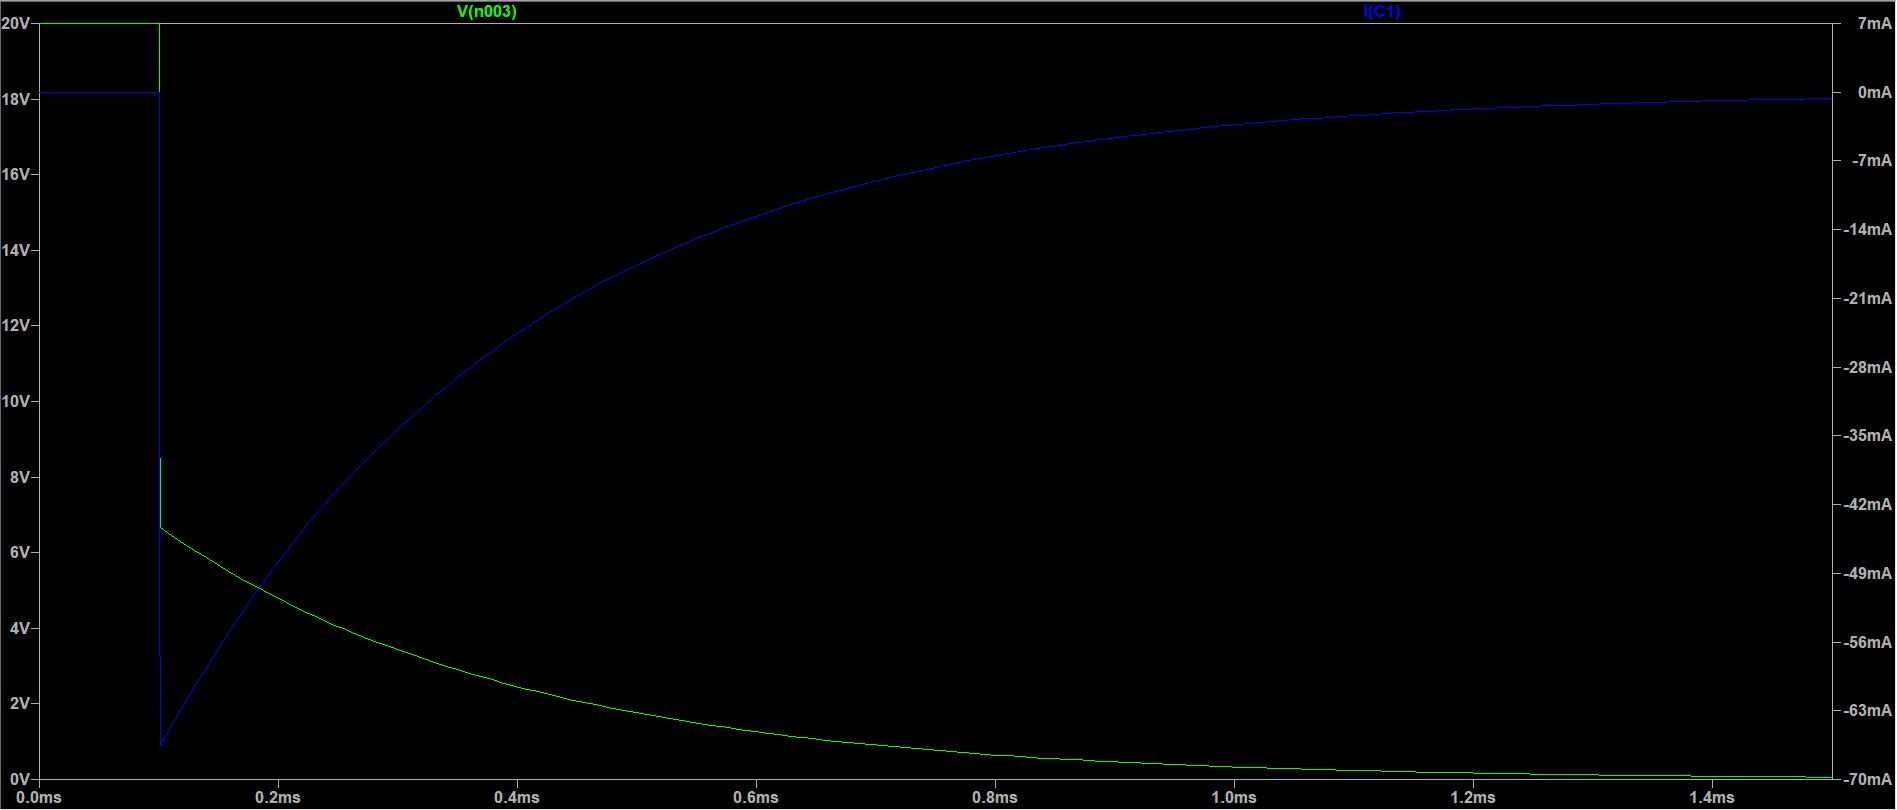
\includegraphics[scale=0.4]{../assets/images/ET2P5/aufgabe 2 u von t und i von t.JPG}
    \caption{Zeiltiche Verläufe von $U_L$ und $I_L$}
  \end{center}
\end{figure}

\subsection{Bestimmung von $\tau$}

\begin{figure}[h]
  \begin{center}
    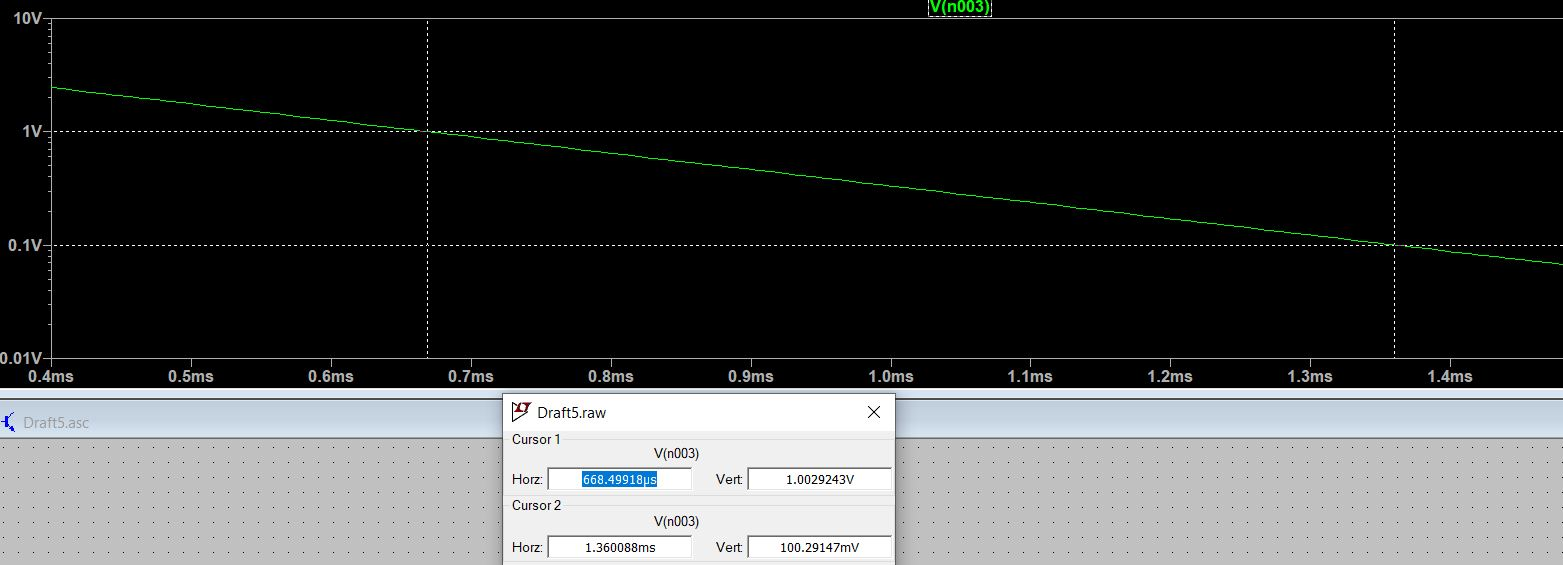
\includegraphics[scale=0.5]{../assets/images/ET2P5/tau log aufgabe 2.JPG}
    \caption{Bestimmung der Zeitkonstante}
  \end{center}
\end{figure}
Die Spannung wird nun logaritmisch dargestellt. Nun werden mittels der Cursor-Funktion zwei Zeitpunkte zu jeweils einer Dekade ermittelt.
Daraus ergibt sich:
\begin{align*}
  \tau &= \frac{t_2-t_1}{ln(10)}\\
  \tau &= \frac{1,36ms - 668,5\mu s}{ln (10)}\\
  \tau &= 300\mu s
\end{align*}


\newpage


\section{Schaltvorgang bei einem Netzwerk mit einer Spule(zwei Schaltzeitpunkte)}
\begin{task}
  In diesem Versuch wollen hier das Verhalten einer Spule in einem Netzwerk untersuchen, die auch wieder von einem Schalter gesteuert wird. Die mathematische Vorbetrachtung wird wieder mit den Simulationsergebnissen verglichen.


\end{task}

\subsection{Simulation der Schaltung}
\begin{figure}[h]
  \begin{center}
    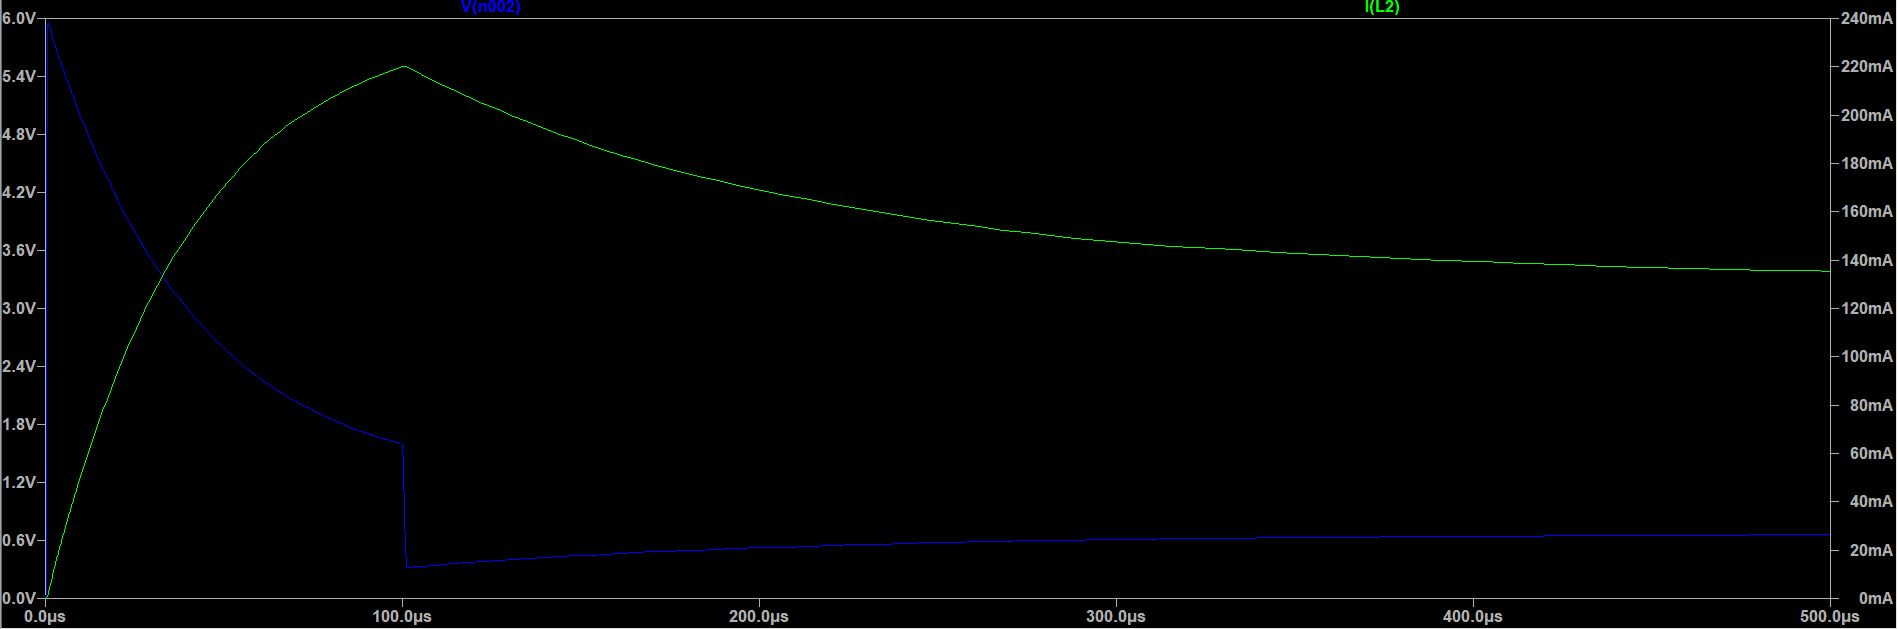
\includegraphics[scale=0.4]{../assets/images/ET2P5/aufgabe 3 u von t und i von t.JPG}
    \caption{Zeiltiche Verläufe von $U_L$ und $I_L$}
  \end{center}
\end{figure}

\subsection{Vergleich der berechneten Werte}

Die Kurven entsprechen den Erwartungen und es lassen sich die vorher berechneten Kenngrößen wiederfinden.

\subsection{Ermittlung der Spannung $u_L$}

Gleichung der Spannung über der Induktivität:

Für den Zeitbereich t0 < t < t1 gilt:
\begin{align*}
  u_L(t) = 6V\cdot e^{-\frac{t}{40\mu s}}\cdot 
\end{align*}
Wenn t1 < 1 gilt für die Spannung:

\begin{align*}
  u_L(t) &= L\cdot \frac{\mathrm{d} i}{\mathrm{d} t}\\
  u_L(t) &= L\cdot (133,33mA + 86,67mA\cdot e^{-\frac{t-100\mu s}{111,1\mu s}})\frac{\mathrm{d} i}{\mathrm{d} t}\\
  u_L(t) &= 1mH\cdot \left(-\frac{1}{111,1\mu s}\cdot 86,67mA\cdot e^{-\frac{t-100\mu s}{111,1\mu s}}\right)\\
  u_L(t) &= -780mV\cdot e^{-\frac{t-100\mu s}{111,1\mu s}}
\end{align*}
\newpage


\end{document}
